% ==========================================================================
\section{Language C: proofs without words (the Nelsen style)}
\label{sec:nelsen}

\paragraph{Marks.} Segments whose \emph{lengths} are the quantities, regions whose
\emph{areas} are the quantities, and arrays whose \emph{counts} are the quantities.
\paragraph{Legal moves.} Dissect and reassemble (area is additive); superimpose two
figures (comparison); rotate or reflect a copy of the figure (symmetry).
\paragraph{Soundness.} None in general. A dissection proves an identity only if the
pieces really do fit -- which is a statement about the generic configuration. The
symbolic residue is: \emph{list the configurations, and check the picture in each}.

\subsection{The triangle inequality itself}

\begin{figure}[H]
\centering
\begin{tikzpicture}[x=1cm,y=1cm]
  % same sign
  \draw[axis] (0,0) -- (5.4,0);
  \fill (0.4,0) circle (1.4pt) node[below=2pt,font=\scriptsize]{$0$};
  \draw[vec,blue!60!black] (0.4,0.3) -- node[above,font=\scriptsize]{$a$} (2.4,0.3);
  \draw[vec,red!60!black] (2.4,0.3) -- node[above,font=\scriptsize]{$b$} (4.4,0.3);
  \draw[decorate,decoration={brace,amplitude=4pt,mirror}] (0.4,-0.25) -- (4.4,-0.25)
     node[midway,below,font=\scriptsize]{$|a+b|=|a|+|b|$};
  \node[font=\scriptsize] at (2.6,1.1) {same direction};
  % opposite sign
  \begin{scope}[xshift=6.6cm]
  \draw[axis] (0,0) -- (5.4,0);
  \fill (0.4,0) circle (1.4pt) node[below=2pt,font=\scriptsize]{$0$};
  \draw[vec,blue!60!black] (0.4,0.3) -- node[above,font=\scriptsize]{$a$} (4.4,0.3);
  \draw[vec,red!60!black] (4.4,0.75) -- node[above,font=\scriptsize]{$b$} (2.4,0.75);
  \draw[decorate,decoration={brace,amplitude=4pt,mirror}] (0.4,-0.25) -- (2.4,-0.25)
     node[midway,below,font=\scriptsize]{$|a+b|<|a|+|b|$};
  \node[font=\scriptsize] at (2.6,1.35) {opposite directions};
  \end{scope}
\end{tikzpicture}
\caption{$|a+b|\le|a|+|b|$ on the number line: lay the two displacements head to tail.
If they point the same way the lengths add; if they point opposite ways they partly
cancel. \emph{Both} pictures must be drawn -- this is the symbolic residue of the case
distinction $\operatorname{sign}a=\operatorname{sign}b$ or not. Certified (in the general
form of exercise 1.13) in \lean{DiagramProofs.abs\_sum\_range\_le\_sum\_abs}.}
\label{fig:absline}
\end{figure}

\begin{figure}[H]
\centering
\begin{tikzpicture}[x=1cm,y=1cm]
  \coordinate (O) at (0,0);
  \coordinate (U) at (2.6,1.4);
  \coordinate (V) at (1.5,-0.9);
  \coordinate (S) at ($(U)+(V)$);
  \draw[gray,dashed] (U) -- (S) -- (V);
  \draw[vec,blue!60!black] (O) -- node[above left,font=\scriptsize]{$u$} (U);
  \draw[vec,red!60!black] (O) -- node[below,font=\scriptsize]{$v$} (V);
  \draw[vec] (O) -- node[right,font=\scriptsize,pos=0.75]{$u+v$} (S);
  \draw[vec,red!60!black] (U) -- node[above right,font=\scriptsize]{$v$} (S);
  \fill (O) circle (1.5pt);
\end{tikzpicture}
\hspace{1.2cm}
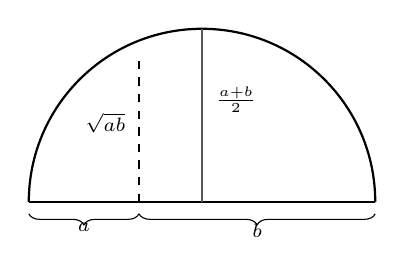
\begin{tikzpicture}[x=1cm,y=1cm]
  \draw[thick] (0,0) -- (4.4,0);
  \draw[thick] (0,0) arc (180:0:2.2);
  \coordinate (P) at (1.4,0);
  \draw[dashed] (P) -- (1.4,1.83);
  \draw[thick,gray!70!black] (2.2,0) -- (2.2,2.2);
  \draw[decorate,decoration={brace,amplitude=4pt,mirror}] (0,-0.15) -- (1.4,-0.15)
      node[midway,below,font=\scriptsize]{$a$};
  \draw[decorate,decoration={brace,amplitude=4pt,mirror}] (1.4,-0.15) -- (4.4,-0.15)
      node[midway,below,font=\scriptsize]{$b$};
  \node[font=\scriptsize,anchor=east] at (1.35,1.0) {$\sqrt{ab}$};
  \node[font=\scriptsize,anchor=west] at (2.25,1.3) {$\frac{a+b}{2}$};
\end{tikzpicture}
\caption{Left: the triangle inequality in the plane -- the parallelogram picture of
$\norm{u+v}\le\norm{u}+\norm{v}$ (\lean{DiagramProofs.norm\_add\_le'}). Right: the
archetypal proof without words. In a semicircle of diameter $a+b$ the altitude over the
splitting point has length $\sqrt{ab}$ and the radius has length $(a+b)/2$; an altitude
is at most a radius, so $\sqrt{ab}\le\frac{a+b}{2}$
(\lean{DiagramProofs.sqrt\_mul\_le\_add\_div\_two}).}
\label{fig:amgm}
\end{figure}

\subsection{Cauchy--Schwarz as a picture}

\begin{figure}[H]
\centering
\begin{tikzpicture}[x=1cm,y=1cm]
  \coordinate (O) at (0,0);
  \coordinate (U) at (3.4,0);
  \coordinate (V) at (2.0,1.7);
  \draw[vec] (O) -- node[below,font=\scriptsize]{$u$} (U);
  \draw[vec] (O) -- node[above left,font=\scriptsize]{$v$} (V);
  \draw[dashed] (V) -- (2.0,0);
  \draw[decorate,decoration={brace,amplitude=4pt}] (0,-0.6) -- (2.0,-0.6)
     node[midway,below,font=\scriptsize]{$\dfrac{\langle u,v\rangle}{\norm{u}}
       =\norm{v}\cos\theta\ \le\ \norm{v}$};
  \draw (0.55,0) arc (0:40:0.55);
  \node[font=\scriptsize] at (0.85,0.24) {$\theta$};
\end{tikzpicture}
\caption{Cauchy--Schwarz, $|\langle u,v\rangle|\le\norm{u}\norm{v}$: the projection of
$v$ onto the line of $u$ is never longer than $v$ itself. The only fact used is that in a
right triangle the leg is at most the hypotenuse -- itself a triangle-inequality picture.
Certified in \lean{TriangleOverlap.cauchy\_schwarz}.}
\label{fig:cs}
\end{figure}

\subsection{Sums: exercises 1.14 and 1.16}

\begin{figure}[H]
\centering
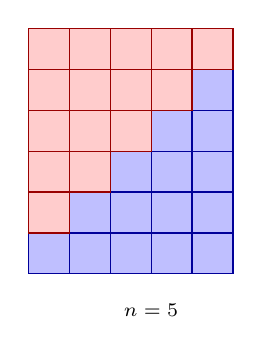
\begin{tikzpicture}[x=0.52cm,y=0.52cm]
  \foreach \i in {1,...,5}{
    \foreach \j in {1,...,\i}{
      \fill[blue!25,draw=blue!60!black] (\i-1,\j-1) rectangle (\i,\j);}}
  \foreach \i in {1,...,5}{
    \foreach \j in {1,...,\i}{
      \fill[red!20,draw=red!60!black] (5-\i,6-\j) rectangle (6-\i,7-\j);}}
  \node[font=\scriptsize] at (3,-0.9) {$n=5$};
\end{tikzpicture}
\hspace{1.3cm}
\begin{tikzpicture}[x=0.62cm,y=0.62cm,baseline=(current bounding box.center)]
  \foreach \i/\v in {1/1,2/2,3/3,4/4}{
    \foreach \j in {1,...,\i}{
      \node[font=\scriptsize] at ({\j-\i/2},{-\i}) {$\v$};}}
  \node[font=\scriptsize,gray] at (0,-5.1) {rotate twice, add: every cell shows $2n+1$};
\end{tikzpicture}
\caption{Left: $1+2+\dots+n$ twice over tiles an $n\times(n+1)$ rectangle, so the sum is
$n(n+1)/2$ (exercise 1.14 a). Right: the triangular array with $i$ copies of $i$ in row
$i$ has sum $\sum i^2$; superimposing the array with its two $120^\circ$ rotations makes
every cell equal to $2n+1$, and the array has $n(n+1)/2$ cells, so
$3\sum i^{2}=(2n+1)\,n(n+1)/2$ -- exercise 1.16, ``bizony\'{\i}t\'as szavak n\'elk\"ul''.
Certified in \lean{DiagramProofs.six\_mul\_sum\_sq}.}
\label{fig:sums}
\end{figure}

\begin{figure}[H]
\centering
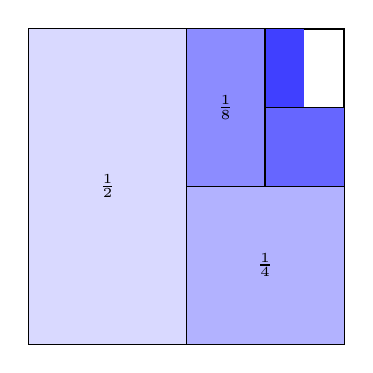
\begin{tikzpicture}[x=4cm,y=4cm]
  \draw[thick] (0,0) rectangle (1,1);
  \fill[blue!15] (0,0) rectangle (0.5,1);
  \fill[blue!30] (0.5,0) rectangle (1,0.5);
  \fill[blue!45] (0.5,0.5) rectangle (0.75,1);
  \fill[blue!60] (0.75,0.5) rectangle (1,0.75);
  \fill[blue!75] (0.75,0.75) rectangle (0.875,1);
  \draw (0.5,0) -- (0.5,1); \draw (0.5,0.5) -- (1,0.5);
  \draw (0.75,0.5) -- (0.75,1); \draw (0.75,0.75) -- (1,0.75);
  \node[font=\scriptsize] at (0.25,0.5) {$\frac12$};
  \node[font=\scriptsize] at (0.75,0.25) {$\frac14$};
  \node[font=\scriptsize] at (0.625,0.75) {$\frac18$};
\end{tikzpicture}
\caption{The frog of exercise 1.6 (and the geometric series of 1.14 c with $q=\frac12$):
the halves of the unit square exhaust it, so $\frac12+\frac14+\frac18+\dots=1$. What the
picture shows rigorously is that every \emph{partial} sum is $1-2^{-n}<1$; that the limit
is exactly $1$ is the symbolic residue, and it is where the notion of limit enters. The
frog gets the kiss only in the limit.}
\label{fig:geom}
\end{figure}

\begin{trap}[A dissection can lie]
Rearranging the four pieces of an $8\times8$ square into a $5\times13$ rectangle
``shows'' $64=65$; the pieces overlap along a sliver of area $1$ that is invisible at
drawing accuracy. A dissection is a proof only when the incidences it assumes are
verified -- here, that three points are collinear, which is false. Rule: \emph{a picture
may assert equalities of areas and lengths, never incidences}.
\end{trap}
